% Arquitectura del perceptron multicapa (MLP).
%
% Fragmento para % Arquitectura del perceptron multicapa (MLP).
%
% Fragmento para % Arquitectura del perceptron multicapa (MLP).
%
% Fragmento para % Arquitectura del perceptron multicapa (MLP).
%
% Fragmento para \input{Figures/mlp_arquitectura}.
% Requiere en el preambulo del documento principal:
%   \usepackage{tikz}
%   \usetikzlibrary{decorations.pathreplacing}
%   \usepackage{amsmath,amssymb}
%
% Entradas (63): pa_1..pa_22, pr_1..pr_37, power, caudal, temperatura, presion.
% Salidas (2):   MDNBR, void.
% h = hidden_dim, L = cantidad de bloques lineal+activacion repetidos,
% sigma = funcion de activacion.
% La red tiene L+1 capas ocultas: la primera proviene de la capa lineal de
% entrada y las L restantes del bloque repetido.

\begin{figure}[htbp]
  \centering
  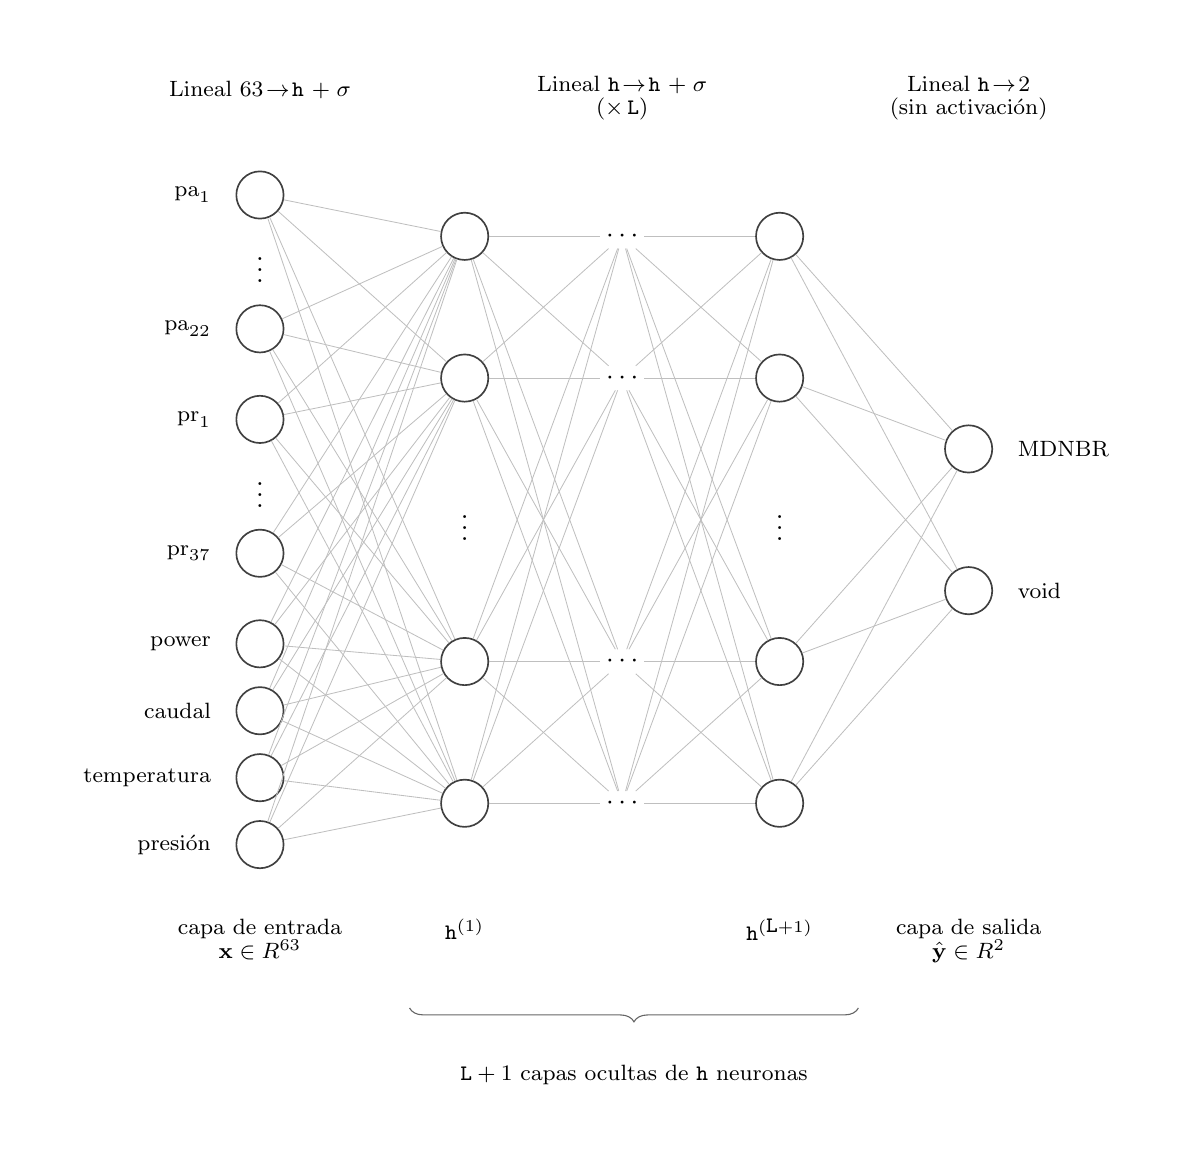
\begin{tikzpicture}[
      neurona/.style  = {circle, draw=black!75, fill=white, line width=0.6pt,
                         minimum size=6mm, inner sep=0pt},
      conexion/.style = {draw=black!25, line width=0.3pt},
      puntos/.style   = {inner sep=2pt},
      nombre/.style   = {font=\footnotesize},
      texto/.style    = {font=\footnotesize, align=center},
    ]
    \useasboundingbox (-2.95,-7.7) rectangle (11.6,6.25);

    %------------------------------------------------ capa de entrada (63)
    \foreach \y/\etq [count=\i] in {%
        4.125/$\mathrm{pa}_{1}$,
        2.425/$\mathrm{pa}_{22}$,
        1.275/$\mathrm{pr}_{1}$,
        -0.425/$\mathrm{pr}_{37}$,
        -1.575/power,
        -2.425/caudal,
        -3.275/temperatura,
        -4.125/presi\'on} {
      \node[neurona] (I-\i) at (0,\y) {};
      \node[nombre, anchor=east] at (-0.5,\y) {\etq};
    }
    \node[puntos] at (0,3.275) {$\vdots$};
    \node[puntos] at (0,0.425) {$\vdots$};

    %------------------------------------------------ primera capa oculta
    \foreach \y [count=\i] in {3.6, 1.8, -1.8, -3.6}
      \node[neurona] (H-\i) at (2.6,\y) {};
    \node[puntos] at (2.6,0) {$\vdots$};

    %------------------------------------------------ capas ocultas elididas
    \foreach \y [count=\i] in {3.6, 1.8, -1.8, -3.6}
      \node[puntos] (D-\i) at (4.6,\y) {$\cdots$};

    %------------------------------------------------ ultima capa oculta
    \foreach \y [count=\i] in {3.6, 1.8, -1.8, -3.6}
      \node[neurona] (G-\i) at (6.6,\y) {};
    \node[puntos] at (6.6,0) {$\vdots$};

    %------------------------------------------------ capa de salida (2)
    \foreach \y/\etq [count=\i] in {0.9/MDNBR, -0.9/void} {
      \node[neurona] (O-\i) at (9.0,\y) {};
      \node[nombre, anchor=west] at (9.5,\y) {\etq};
    }

    %------------------------------------------------ conexiones densas
    \foreach \a in {1,...,8}
      \foreach \b in {1,...,4}
        \draw[conexion] (I-\a) -- (H-\b);
    \foreach \a in {1,...,4}
      \foreach \b in {1,...,4} {
        \draw[conexion] (H-\a) -- (D-\b);
        \draw[conexion] (D-\a) -- (G-\b);
      }
    \foreach \a in {1,...,4}
      \foreach \b in {1,2}
        \draw[conexion] (G-\a) -- (O-\b);

    %------------------------------------------------ transformaciones
    \node[texto, anchor=south] at (0,4.95)
      {Lineal $63\!\to\!\texttt{h}$ $+\;\sigma$\\[-1pt]};
    \node[texto, anchor=south] at (4.6,4.95)
      {Lineal $\texttt{h}\!\to\!\texttt{h}$ $+\;\sigma$\\[-1pt] ($\times\,\texttt{L}$)};
    \node[texto, anchor=south] at (9,4.95)
      {Lineal $\texttt{h}\!\to\!2$\\[-1pt] (sin activaci\'on)};

    %------------------------------------------------ nombres de las capas
    \node[texto, anchor=north] at (0,-4.95)
      {capa de entrada\\[-1pt] $\mathbf{x}\in\mathbb{R}^{63}$};
    \node[texto, anchor=north] at (2.6,-4.95) {$\mathbf{\texttt{h}}^{(1)}$};
    \node[texto, anchor=north] at (6.6,-4.95) {$\mathbf{\texttt{h}}^{(\texttt{L}+1)}$};
    \node[texto, anchor=north] at (9.0,-4.95)
      {capa de salida\\[-1pt] $\hat{\mathbf{y}}\in\mathbb{R}^{2}$};

    %------------------------------------------------ llave de capas ocultas
    \draw[decorate, decoration={brace, amplitude=5pt, mirror}, draw=black!60]
      (1.9,-6.2) -- (7.6,-6.2);
    \node[texto, anchor=north] at (4.75,-6.8)
      {$\texttt{L}+1$ capas ocultas de \texttt{h} neuronas};
  \end{tikzpicture}
  \caption{Arquitectura de la DNN para estimación de MDNBR y fracción de vacío, para predicción de PLC.}
  \label{fig:mlp-arquitectura}
\end{figure}
.
% Requiere en el preambulo del documento principal:
%   \usepackage{tikz}
%   \usetikzlibrary{decorations.pathreplacing}
%   \usepackage{amsmath,amssymb}
%
% Entradas (63): pa_1..pa_22, pr_1..pr_37, power, caudal, temperatura, presion.
% Salidas (2):   MDNBR, void.
% h = hidden_dim, L = cantidad de bloques lineal+activacion repetidos,
% sigma = funcion de activacion.
% La red tiene L+1 capas ocultas: la primera proviene de la capa lineal de
% entrada y las L restantes del bloque repetido.

\begin{figure}[htbp]
  \centering
  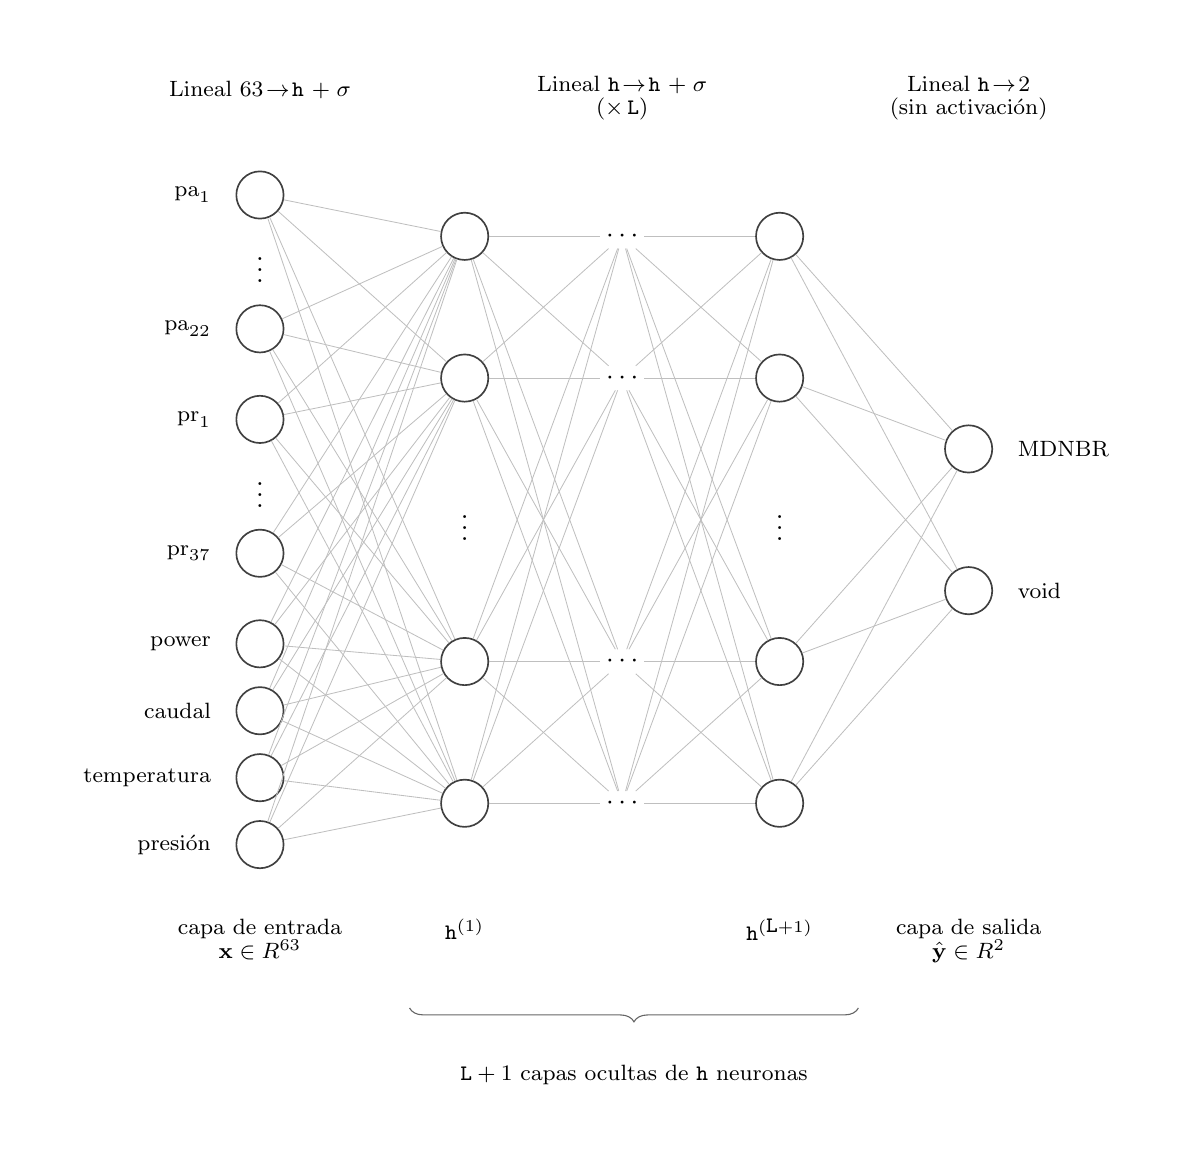
\begin{tikzpicture}[
      neurona/.style  = {circle, draw=black!75, fill=white, line width=0.6pt,
                         minimum size=6mm, inner sep=0pt},
      conexion/.style = {draw=black!25, line width=0.3pt},
      puntos/.style   = {inner sep=2pt},
      nombre/.style   = {font=\footnotesize},
      texto/.style    = {font=\footnotesize, align=center},
    ]
    \useasboundingbox (-2.95,-7.7) rectangle (11.6,6.25);

    %------------------------------------------------ capa de entrada (63)
    \foreach \y/\etq [count=\i] in {%
        4.125/$\mathrm{pa}_{1}$,
        2.425/$\mathrm{pa}_{22}$,
        1.275/$\mathrm{pr}_{1}$,
        -0.425/$\mathrm{pr}_{37}$,
        -1.575/power,
        -2.425/caudal,
        -3.275/temperatura,
        -4.125/presi\'on} {
      \node[neurona] (I-\i) at (0,\y) {};
      \node[nombre, anchor=east] at (-0.5,\y) {\etq};
    }
    \node[puntos] at (0,3.275) {$\vdots$};
    \node[puntos] at (0,0.425) {$\vdots$};

    %------------------------------------------------ primera capa oculta
    \foreach \y [count=\i] in {3.6, 1.8, -1.8, -3.6}
      \node[neurona] (H-\i) at (2.6,\y) {};
    \node[puntos] at (2.6,0) {$\vdots$};

    %------------------------------------------------ capas ocultas elididas
    \foreach \y [count=\i] in {3.6, 1.8, -1.8, -3.6}
      \node[puntos] (D-\i) at (4.6,\y) {$\cdots$};

    %------------------------------------------------ ultima capa oculta
    \foreach \y [count=\i] in {3.6, 1.8, -1.8, -3.6}
      \node[neurona] (G-\i) at (6.6,\y) {};
    \node[puntos] at (6.6,0) {$\vdots$};

    %------------------------------------------------ capa de salida (2)
    \foreach \y/\etq [count=\i] in {0.9/MDNBR, -0.9/void} {
      \node[neurona] (O-\i) at (9.0,\y) {};
      \node[nombre, anchor=west] at (9.5,\y) {\etq};
    }

    %------------------------------------------------ conexiones densas
    \foreach \a in {1,...,8}
      \foreach \b in {1,...,4}
        \draw[conexion] (I-\a) -- (H-\b);
    \foreach \a in {1,...,4}
      \foreach \b in {1,...,4} {
        \draw[conexion] (H-\a) -- (D-\b);
        \draw[conexion] (D-\a) -- (G-\b);
      }
    \foreach \a in {1,...,4}
      \foreach \b in {1,2}
        \draw[conexion] (G-\a) -- (O-\b);

    %------------------------------------------------ transformaciones
    \node[texto, anchor=south] at (0,4.95)
      {Lineal $63\!\to\!\texttt{h}$ $+\;\sigma$\\[-1pt]};
    \node[texto, anchor=south] at (4.6,4.95)
      {Lineal $\texttt{h}\!\to\!\texttt{h}$ $+\;\sigma$\\[-1pt] ($\times\,\texttt{L}$)};
    \node[texto, anchor=south] at (9,4.95)
      {Lineal $\texttt{h}\!\to\!2$\\[-1pt] (sin activaci\'on)};

    %------------------------------------------------ nombres de las capas
    \node[texto, anchor=north] at (0,-4.95)
      {capa de entrada\\[-1pt] $\mathbf{x}\in\mathbb{R}^{63}$};
    \node[texto, anchor=north] at (2.6,-4.95) {$\mathbf{\texttt{h}}^{(1)}$};
    \node[texto, anchor=north] at (6.6,-4.95) {$\mathbf{\texttt{h}}^{(\texttt{L}+1)}$};
    \node[texto, anchor=north] at (9.0,-4.95)
      {capa de salida\\[-1pt] $\hat{\mathbf{y}}\in\mathbb{R}^{2}$};

    %------------------------------------------------ llave de capas ocultas
    \draw[decorate, decoration={brace, amplitude=5pt, mirror}, draw=black!60]
      (1.9,-6.2) -- (7.6,-6.2);
    \node[texto, anchor=north] at (4.75,-6.8)
      {$\texttt{L}+1$ capas ocultas de \texttt{h} neuronas};
  \end{tikzpicture}
  \caption{Arquitectura de la DNN para estimación de MDNBR y fracción de vacío, para predicción de PLC.}
  \label{fig:mlp-arquitectura}
\end{figure}
.
% Requiere en el preambulo del documento principal:
%   \usepackage{tikz}
%   \usetikzlibrary{decorations.pathreplacing}
%   \usepackage{amsmath,amssymb}
%
% Entradas (63): pa_1..pa_22, pr_1..pr_37, power, caudal, temperatura, presion.
% Salidas (2):   MDNBR, void.
% h = hidden_dim, L = cantidad de bloques lineal+activacion repetidos,
% sigma = funcion de activacion.
% La red tiene L+1 capas ocultas: la primera proviene de la capa lineal de
% entrada y las L restantes del bloque repetido.

\begin{figure}[htbp]
  \centering
  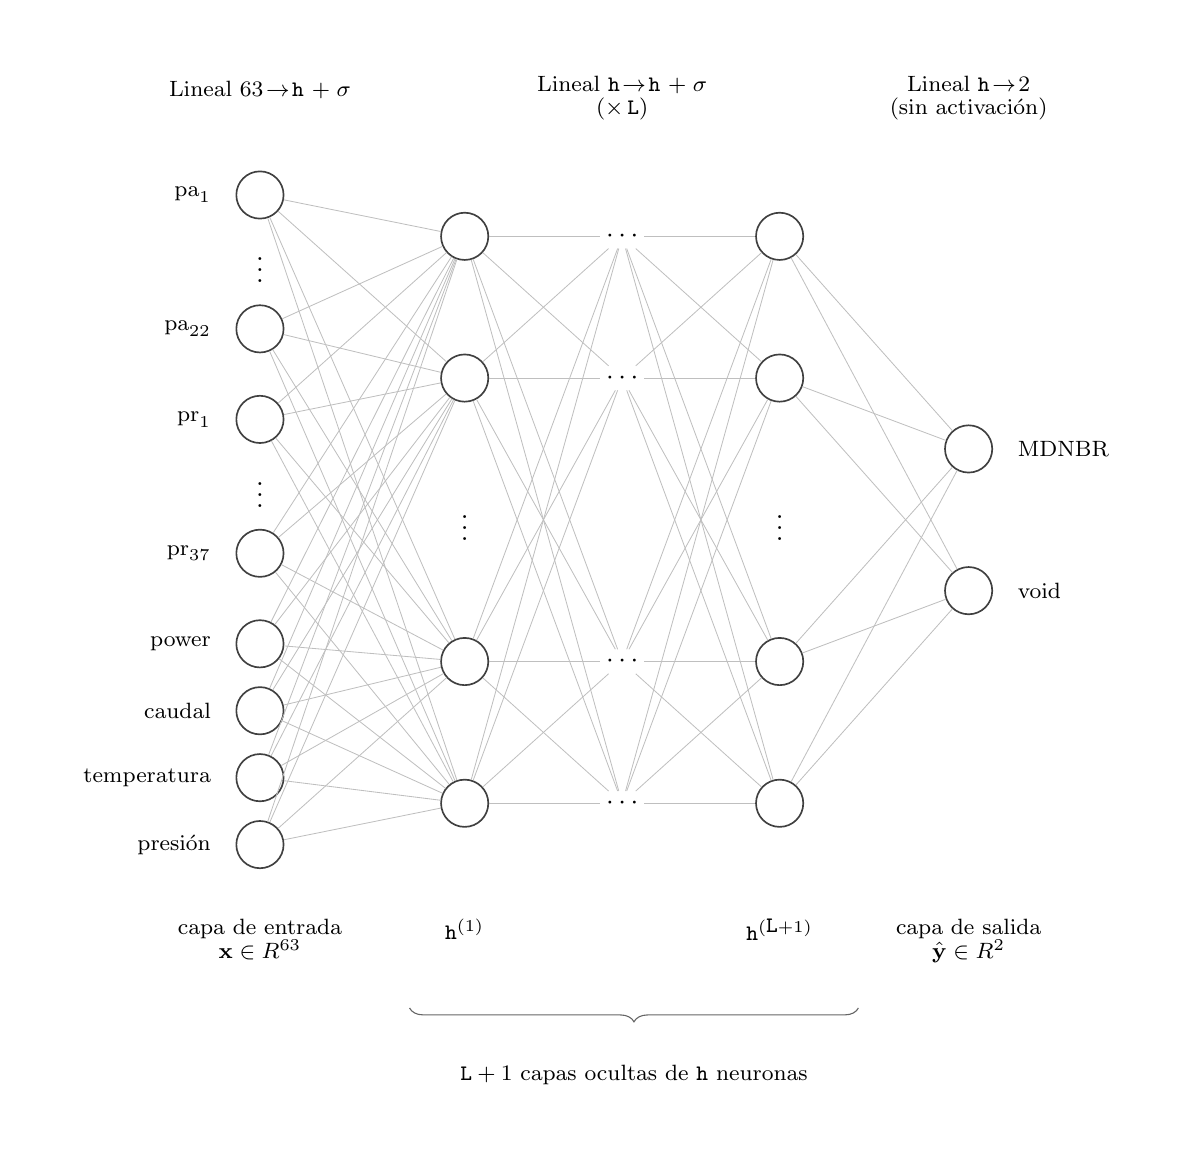
\begin{tikzpicture}[
      neurona/.style  = {circle, draw=black!75, fill=white, line width=0.6pt,
                         minimum size=6mm, inner sep=0pt},
      conexion/.style = {draw=black!25, line width=0.3pt},
      puntos/.style   = {inner sep=2pt},
      nombre/.style   = {font=\footnotesize},
      texto/.style    = {font=\footnotesize, align=center},
    ]
    \useasboundingbox (-2.95,-7.7) rectangle (11.6,6.25);

    %------------------------------------------------ capa de entrada (63)
    \foreach \y/\etq [count=\i] in {%
        4.125/$\mathrm{pa}_{1}$,
        2.425/$\mathrm{pa}_{22}$,
        1.275/$\mathrm{pr}_{1}$,
        -0.425/$\mathrm{pr}_{37}$,
        -1.575/power,
        -2.425/caudal,
        -3.275/temperatura,
        -4.125/presi\'on} {
      \node[neurona] (I-\i) at (0,\y) {};
      \node[nombre, anchor=east] at (-0.5,\y) {\etq};
    }
    \node[puntos] at (0,3.275) {$\vdots$};
    \node[puntos] at (0,0.425) {$\vdots$};

    %------------------------------------------------ primera capa oculta
    \foreach \y [count=\i] in {3.6, 1.8, -1.8, -3.6}
      \node[neurona] (H-\i) at (2.6,\y) {};
    \node[puntos] at (2.6,0) {$\vdots$};

    %------------------------------------------------ capas ocultas elididas
    \foreach \y [count=\i] in {3.6, 1.8, -1.8, -3.6}
      \node[puntos] (D-\i) at (4.6,\y) {$\cdots$};

    %------------------------------------------------ ultima capa oculta
    \foreach \y [count=\i] in {3.6, 1.8, -1.8, -3.6}
      \node[neurona] (G-\i) at (6.6,\y) {};
    \node[puntos] at (6.6,0) {$\vdots$};

    %------------------------------------------------ capa de salida (2)
    \foreach \y/\etq [count=\i] in {0.9/MDNBR, -0.9/void} {
      \node[neurona] (O-\i) at (9.0,\y) {};
      \node[nombre, anchor=west] at (9.5,\y) {\etq};
    }

    %------------------------------------------------ conexiones densas
    \foreach \a in {1,...,8}
      \foreach \b in {1,...,4}
        \draw[conexion] (I-\a) -- (H-\b);
    \foreach \a in {1,...,4}
      \foreach \b in {1,...,4} {
        \draw[conexion] (H-\a) -- (D-\b);
        \draw[conexion] (D-\a) -- (G-\b);
      }
    \foreach \a in {1,...,4}
      \foreach \b in {1,2}
        \draw[conexion] (G-\a) -- (O-\b);

    %------------------------------------------------ transformaciones
    \node[texto, anchor=south] at (0,4.95)
      {Lineal $63\!\to\!\texttt{h}$ $+\;\sigma$\\[-1pt]};
    \node[texto, anchor=south] at (4.6,4.95)
      {Lineal $\texttt{h}\!\to\!\texttt{h}$ $+\;\sigma$\\[-1pt] ($\times\,\texttt{L}$)};
    \node[texto, anchor=south] at (9,4.95)
      {Lineal $\texttt{h}\!\to\!2$\\[-1pt] (sin activaci\'on)};

    %------------------------------------------------ nombres de las capas
    \node[texto, anchor=north] at (0,-4.95)
      {capa de entrada\\[-1pt] $\mathbf{x}\in\mathbb{R}^{63}$};
    \node[texto, anchor=north] at (2.6,-4.95) {$\mathbf{\texttt{h}}^{(1)}$};
    \node[texto, anchor=north] at (6.6,-4.95) {$\mathbf{\texttt{h}}^{(\texttt{L}+1)}$};
    \node[texto, anchor=north] at (9.0,-4.95)
      {capa de salida\\[-1pt] $\hat{\mathbf{y}}\in\mathbb{R}^{2}$};

    %------------------------------------------------ llave de capas ocultas
    \draw[decorate, decoration={brace, amplitude=5pt, mirror}, draw=black!60]
      (1.9,-6.2) -- (7.6,-6.2);
    \node[texto, anchor=north] at (4.75,-6.8)
      {$\texttt{L}+1$ capas ocultas de \texttt{h} neuronas};
  \end{tikzpicture}
  \caption{Arquitectura de la DNN para estimación de MDNBR y fracción de vacío, para predicción de PLC.}
  \label{fig:mlp-arquitectura}
\end{figure}
.
% Requiere en el preambulo del documento principal:
%   \usepackage{tikz}
%   \usetikzlibrary{decorations.pathreplacing}
%   \usepackage{amsmath,amssymb}
%
% Entradas (63): pa_1..pa_22, pr_1..pr_37, power, caudal, temperatura, presion.
% Salidas (2):   MDNBR, void.
% h = hidden_dim, L = cantidad de bloques lineal+activacion repetidos,
% sigma = funcion de activacion.
% La red tiene L+1 capas ocultas: la primera proviene de la capa lineal de
% entrada y las L restantes del bloque repetido.

\begin{figure}[htbp]
  \centering
  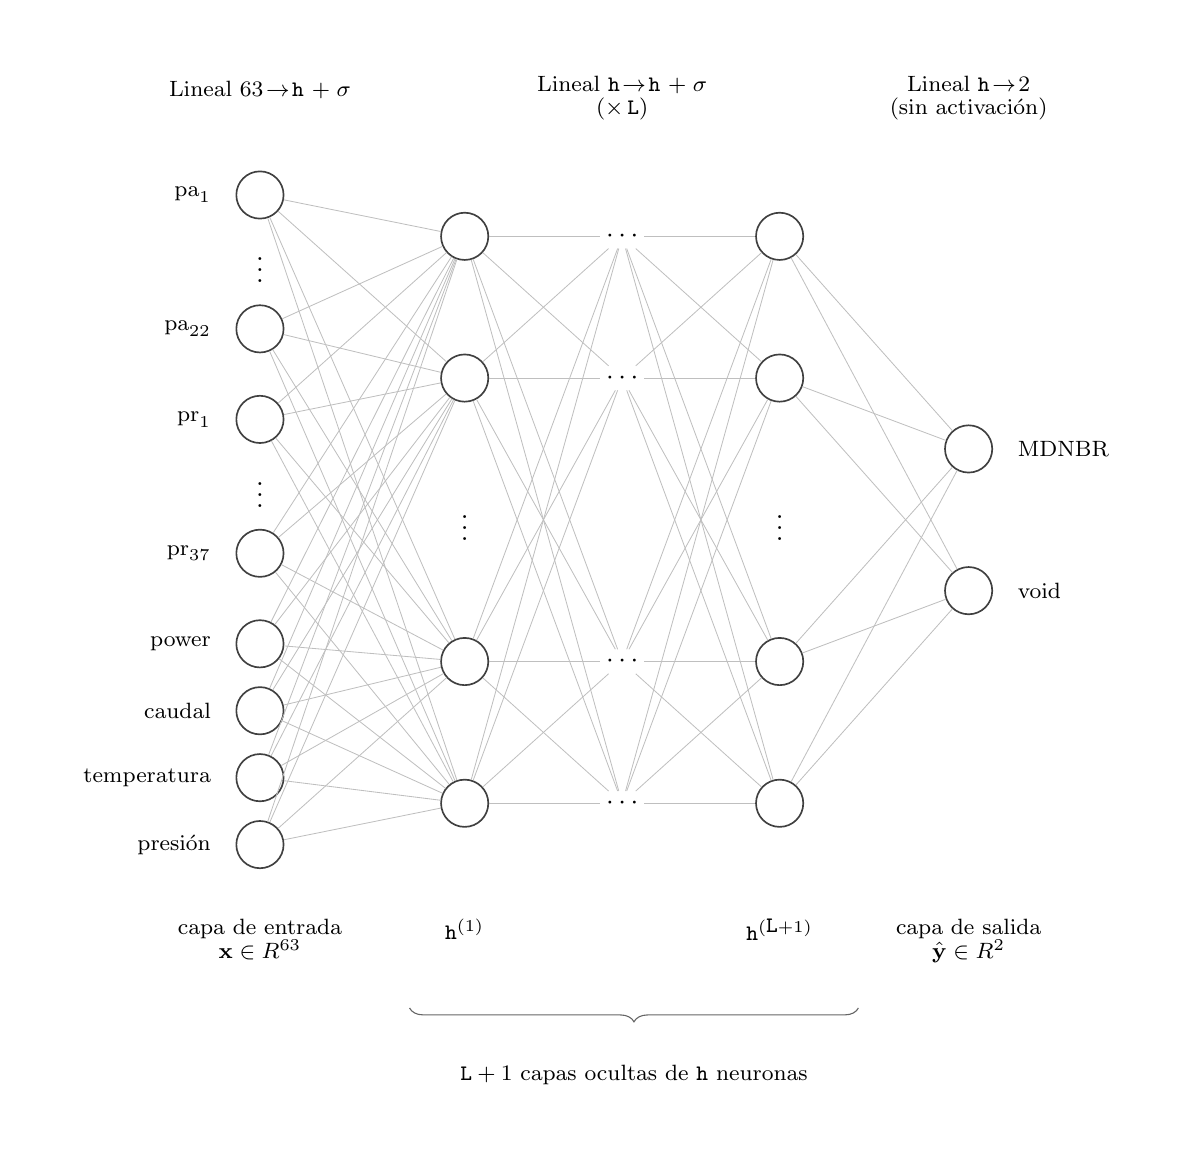
\begin{tikzpicture}[
      neurona/.style  = {circle, draw=black!75, fill=white, line width=0.6pt,
                         minimum size=6mm, inner sep=0pt},
      conexion/.style = {draw=black!25, line width=0.3pt},
      puntos/.style   = {inner sep=2pt},
      nombre/.style   = {font=\footnotesize},
      texto/.style    = {font=\footnotesize, align=center},
    ]
    \useasboundingbox (-2.95,-7.7) rectangle (11.6,6.25);

    %------------------------------------------------ capa de entrada (63)
    \foreach \y/\etq [count=\i] in {%
        4.125/$\mathrm{pa}_{1}$,
        2.425/$\mathrm{pa}_{22}$,
        1.275/$\mathrm{pr}_{1}$,
        -0.425/$\mathrm{pr}_{37}$,
        -1.575/power,
        -2.425/caudal,
        -3.275/temperatura,
        -4.125/presi\'on} {
      \node[neurona] (I-\i) at (0,\y) {};
      \node[nombre, anchor=east] at (-0.5,\y) {\etq};
    }
    \node[puntos] at (0,3.275) {$\vdots$};
    \node[puntos] at (0,0.425) {$\vdots$};

    %------------------------------------------------ primera capa oculta
    \foreach \y [count=\i] in {3.6, 1.8, -1.8, -3.6}
      \node[neurona] (H-\i) at (2.6,\y) {};
    \node[puntos] at (2.6,0) {$\vdots$};

    %------------------------------------------------ capas ocultas elididas
    \foreach \y [count=\i] in {3.6, 1.8, -1.8, -3.6}
      \node[puntos] (D-\i) at (4.6,\y) {$\cdots$};

    %------------------------------------------------ ultima capa oculta
    \foreach \y [count=\i] in {3.6, 1.8, -1.8, -3.6}
      \node[neurona] (G-\i) at (6.6,\y) {};
    \node[puntos] at (6.6,0) {$\vdots$};

    %------------------------------------------------ capa de salida (2)
    \foreach \y/\etq [count=\i] in {0.9/MDNBR, -0.9/void} {
      \node[neurona] (O-\i) at (9.0,\y) {};
      \node[nombre, anchor=west] at (9.5,\y) {\etq};
    }

    %------------------------------------------------ conexiones densas
    \foreach \a in {1,...,8}
      \foreach \b in {1,...,4}
        \draw[conexion] (I-\a) -- (H-\b);
    \foreach \a in {1,...,4}
      \foreach \b in {1,...,4} {
        \draw[conexion] (H-\a) -- (D-\b);
        \draw[conexion] (D-\a) -- (G-\b);
      }
    \foreach \a in {1,...,4}
      \foreach \b in {1,2}
        \draw[conexion] (G-\a) -- (O-\b);

    %------------------------------------------------ transformaciones
    \node[texto, anchor=south] at (0,4.95)
      {Lineal $63\!\to\!\texttt{h}$ $+\;\sigma$\\[-1pt]};
    \node[texto, anchor=south] at (4.6,4.95)
      {Lineal $\texttt{h}\!\to\!\texttt{h}$ $+\;\sigma$\\[-1pt] ($\times\,\texttt{L}$)};
    \node[texto, anchor=south] at (9,4.95)
      {Lineal $\texttt{h}\!\to\!2$\\[-1pt] (sin activaci\'on)};

    %------------------------------------------------ nombres de las capas
    \node[texto, anchor=north] at (0,-4.95)
      {capa de entrada\\[-1pt] $\mathbf{x}\in\mathbb{R}^{63}$};
    \node[texto, anchor=north] at (2.6,-4.95) {$\mathbf{\texttt{h}}^{(1)}$};
    \node[texto, anchor=north] at (6.6,-4.95) {$\mathbf{\texttt{h}}^{(\texttt{L}+1)}$};
    \node[texto, anchor=north] at (9.0,-4.95)
      {capa de salida\\[-1pt] $\hat{\mathbf{y}}\in\mathbb{R}^{2}$};

    %------------------------------------------------ llave de capas ocultas
    \draw[decorate, decoration={brace, amplitude=5pt, mirror}, draw=black!60]
      (1.9,-6.2) -- (7.6,-6.2);
    \node[texto, anchor=north] at (4.75,-6.8)
      {$\texttt{L}+1$ capas ocultas de \texttt{h} neuronas};
  \end{tikzpicture}
  \caption{Arquitectura de la DNN para estimación de MDNBR y fracción de vacío, para predicción de PLC.}
  \label{fig:mlp-arquitectura}
\end{figure}
